\chapter{Validación y Resultados}\label{cap:Validacion}
%Se deben incluir tantos cap\'{\i}tulos como se requieran; sin embargo, se recomienda que la tesis  o trabajo de investigaci\'{o}n tenga un m\'{\i}nimo 3 cap\'{\i}tulos y m\'{a}ximo de 6 cap\'{\i}tulos (incluyendo las conclusiones).\\

%\renewcommand{\tablename}{\textbf{Código}}

En este capítulo se pretende validar el modelo ejecutable que se realiza a partir del esquema preconceptual. Para esto, se programa el modelo ejecutable en C++ \citep{ISO:2017:IIIa}. Se elije este lenguaje porque la \textit{Stardard Template Library} (STL) tiene facilidades que permiten hacer la consistencia del código con el esquema preconceptual explícita, tal como se muestra en la sección \ref{sec:conc++}. Se emula una base de datos a partir de arreglos globales que almacenan cada concepto, y, las claves foráneas que se generan entre conceptos se traducen como punteros. El programa en C++, posteriormente, se valida con un caso de simulación que se usa comúnmente en la literatura, como se expone en la sección \ref{sec:results}.

\section{Traducción a C++ y consistencia}\label{sec:conc++}
A continuación se muestra, a modo de ejemplo, las traducciones de algunos conceptos, funciones, o porciones del EP a código C++ para verificar la consistencia del código con el modelo ejecutable. Primero, se definen los elementos que conforman las condiciones iniciales, y, la base de datos que se emula, es decir, los arreglos que contienen los conceptos que se instancian en la ejecución de las relaciones dinámicas del EP. Posteriormente, se muestran las traducciones a código de dos conceptos clase, ``Malla'' y ``Roca'', y la traducción de la relación dinámica ``Petrofísico caracteriza Roca''. Luego, se explica la traducción del cálculo del residual en el evento ``Presión del Fluido Varía''.\\

Las condiciones iniciales, en las que se definen variables globales y constantes, se programan en un \textit{namespace} ``Global'' que agrupa todas las definiciones, tal como aparecen en la figura \ref{fig:EjInitialConditions}. El código para las condiciones iniciales se expone en la tabla \ref{tab:InitialConditions}.\\

\begin{table}[h]
	\centering
	\begin{tabular}{cc}
		\parbox[c]{10em}{
			\begin{tabular}[c]{@{}c@{}}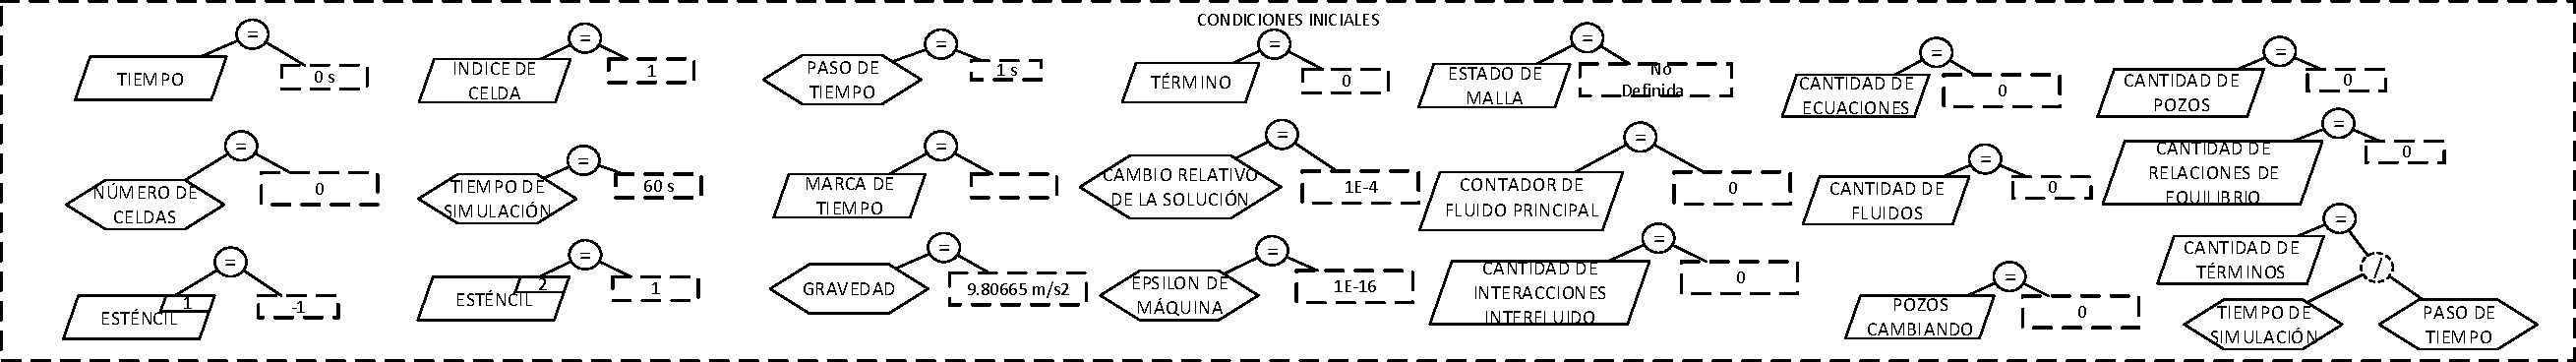
\includegraphics[width=3in]{Fig/EjInitialConditions.pdf}\\ Ver figura \ref{fig:EjInitialConditions}.\end{tabular}
			%
			%\caption[Elementos para la representación de Software Científico.]{Elementos para la representación de Software Científico. \citep{JCalle,norena2018det}.} \label{fig:RockTranslation}
		}
		&
		\begin{tiny}
			\begin{lstlisting}
			namespace Global{
			
			std::string timestamp="";
			double mytime=0;
			double simulationtime = 86400;
			double timedelta=1;
			int wells_quantity=0;
			int term=0;
			int fluids_quantity=0;
			int stencil[2] = {-1,1};
			int equilibrium_relations_quantity=0;
			int interfluid_interactions_quantity=0;
			int cells_number=0;
			int changing_wells=0;
			
			};
			
			
			\end{lstlisting}
		\end{tiny}
	\end{tabular}
	\label{tab:InitialConditions}
	\caption[Traducción a código de las condiciones iniciales.]{Traducción a código de las condiciones iniciales. Los autores.}
\end{table}

En el código \ref{tab:bd} se muestra los conceptos que se almacenan en arreglos, estos se iteran en diferentes funciones del código. Es importante notar que, en las precondiciones del EP se establece que sólo se define una única malla y sólo se caracteriza una única roca. Por tanto, en la base de datos que se emula, estos dos conceptos se acceden por medio de un puntero único. También se destaca que, todos los objetos que se instancian de los conceptos clase, se acceden a partir de punteros. Todos los punteros se fundamentan en la STL, que se encarga de hacer la respectiva gestión del uso de la memoria.\\

\begin{table}
	\begin{tabular}{c}
		\begin{tiny}
			\begin{lstlisting}
			
			std::vector<std::shared_ptr<Equation_Base>> equations =
			std::vector<std::shared_ptr<Equation_Base>>();
			
			std::vector<std::shared_ptr<Fluid>> characterized_fluids =
			std::vector<std::shared_ptr<Fluid>>();
			
			std::vector<std::unique_ptr<Equilibrium_Relation>> added_equilibrium_relations =
			std::vector<std::unique_ptr<Equilibrium_Relation>>();
			
			std::vector<std::unique_ptr<Interfluid_Interaction>> added_interfluid_interactions =
			std::vector<std::unique_ptr<Interfluid_Interaction>>();
			
			std::vector<std::shared_ptr<Well>> perforated_wells =
			std::vector<std::shared_ptr<Well>>();
			
			std::unique_ptr<Mesh> mymesh;
			std::unique_ptr<Rock> myrock;
			
			\end{lstlisting}
		\end{tiny}
	\end{tabular}
	\label{tab:bd}
	\caption[Arreglos que conforman la base de datos que se emula.]{Arreglos que conforman la base de datos que se emula. Los autores.}
\end{table}

En el código \ref{tab:MeshCode} se puede observar que, la conceptualización de la malla coincide con el código que se genera para la misma. La malla se propone como un conjunto de celdas. Adicionalmente, se tienen elementos como el espesor que dependen de la cantidad de celdas en cada dirección. Las celdas también se iteran, pero su arreglo correspondiente se almacena dentro del concepto malla, tal como se propone en la sección \ref{sec:Mesh}(Ojo, hay que ponerle un label que mande a revisar la conceptualización de la malla).

\begin{table}[h]
	\centering
	\begin{tabular}{cc}
		\parbox[c]{5em}{
			\begin{tabular}[c]{@{}c@{}}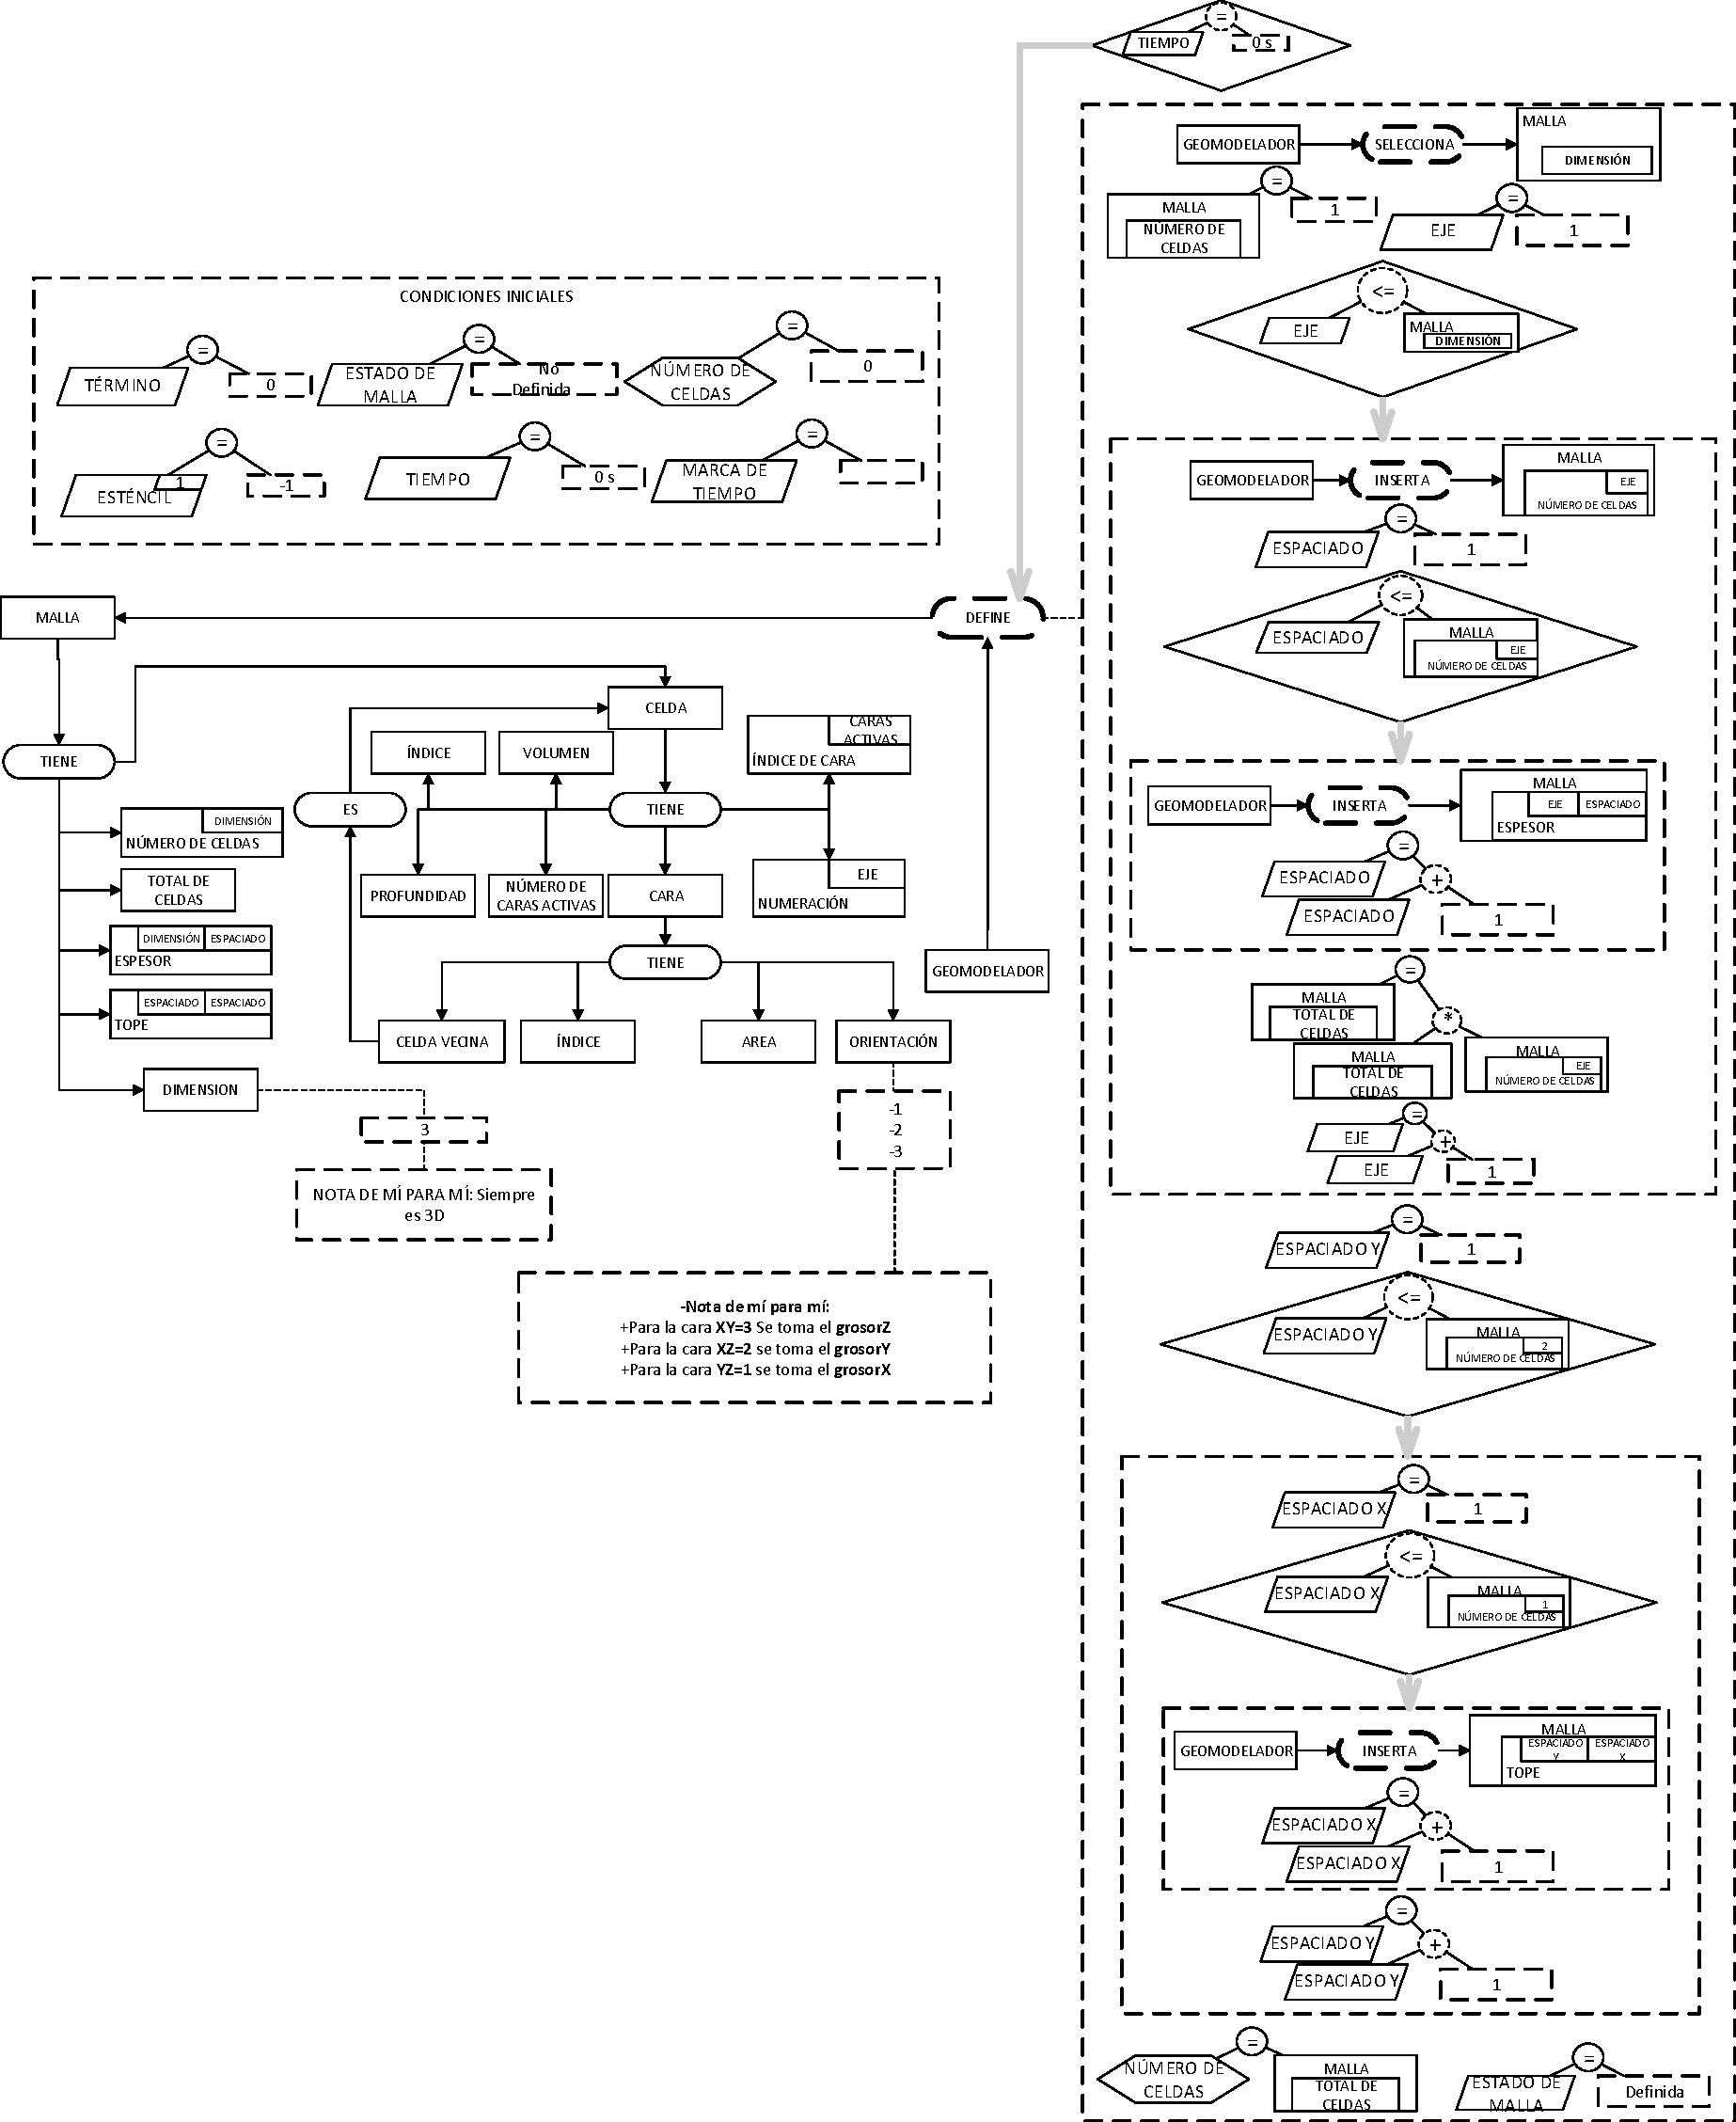
\includegraphics[width=2in]{Fig/Mesh.pdf}\\ Ver figura \ref{fig:Mesh}.\end{tabular}
			%
			%\caption[Elementos para la representación de Software Científico.]{Elementos para la representación de Software Científico. \citep{JCalle,norena2018det}.} \label{fig:RockTranslation}
		}
		&
		\begin{tiny}
			\begin{lstlisting}
			
			class Mesh{
			
			private:
			
			using Cells_t = std::vector<std::shared_ptr<Cell>>;
			int _dimension;
			std::vector<int> _cell_number = std::vector<int>(3);
			int _cell_total;
			std::vector<std::vector<double>> _thickness;
			std::vector<std::vector<double>> _top;
			int _defined=0;
			Cells_t _cells;
			
			public:
			
			using Cell_iterator = Cells_t::iterator;
			using Cell_const_iterator = Cells_t::const_iterator;
			
			Mesh();
			int getCellTotal();
			void define();
			void defineFromFile(std::ifstream& mesh_reader);
			void appear(const std::string& _timestamp, const int stencil[2]);

			int listCell(int posx, int posy, int posz);
			int listCell(std::vector<int> _Numeration);
			
			const std::shared_ptr<Cell>& cell(const int index) const 
			{return _cells[index];};
			
			const double& thickness(const int axis, const int spacing) const 
			{return _thickness[axis][spacing];};
			
			Cell_iterator begin() {return _cells.begin();};
			Cell_iterator end()   {return _cells.end();};
			
			Cell_const_iterator begin()  const {return _cells.begin();};
			Cell_const_iterator end()    const {return _cells.end();};
			Cell_const_iterator cbegin() const {return _cells.cbegin();};
			Cell_const_iterator cend()   const {return _cells.cend();};
			

			};
			
			\end{lstlisting}
		\end{tiny}
	\end{tabular}
	\label{tab:MeshCode}
	\caption[Traducción a código del concepto Malla.]{Traducción a código del concepto Malla. Los autores.}
\end{table}



\begin{table}[h]
	\centering
	\begin{tabular}{cc}
		\parbox[c]{1em}{
			\begin{tabular}[c]{@{}c@{}}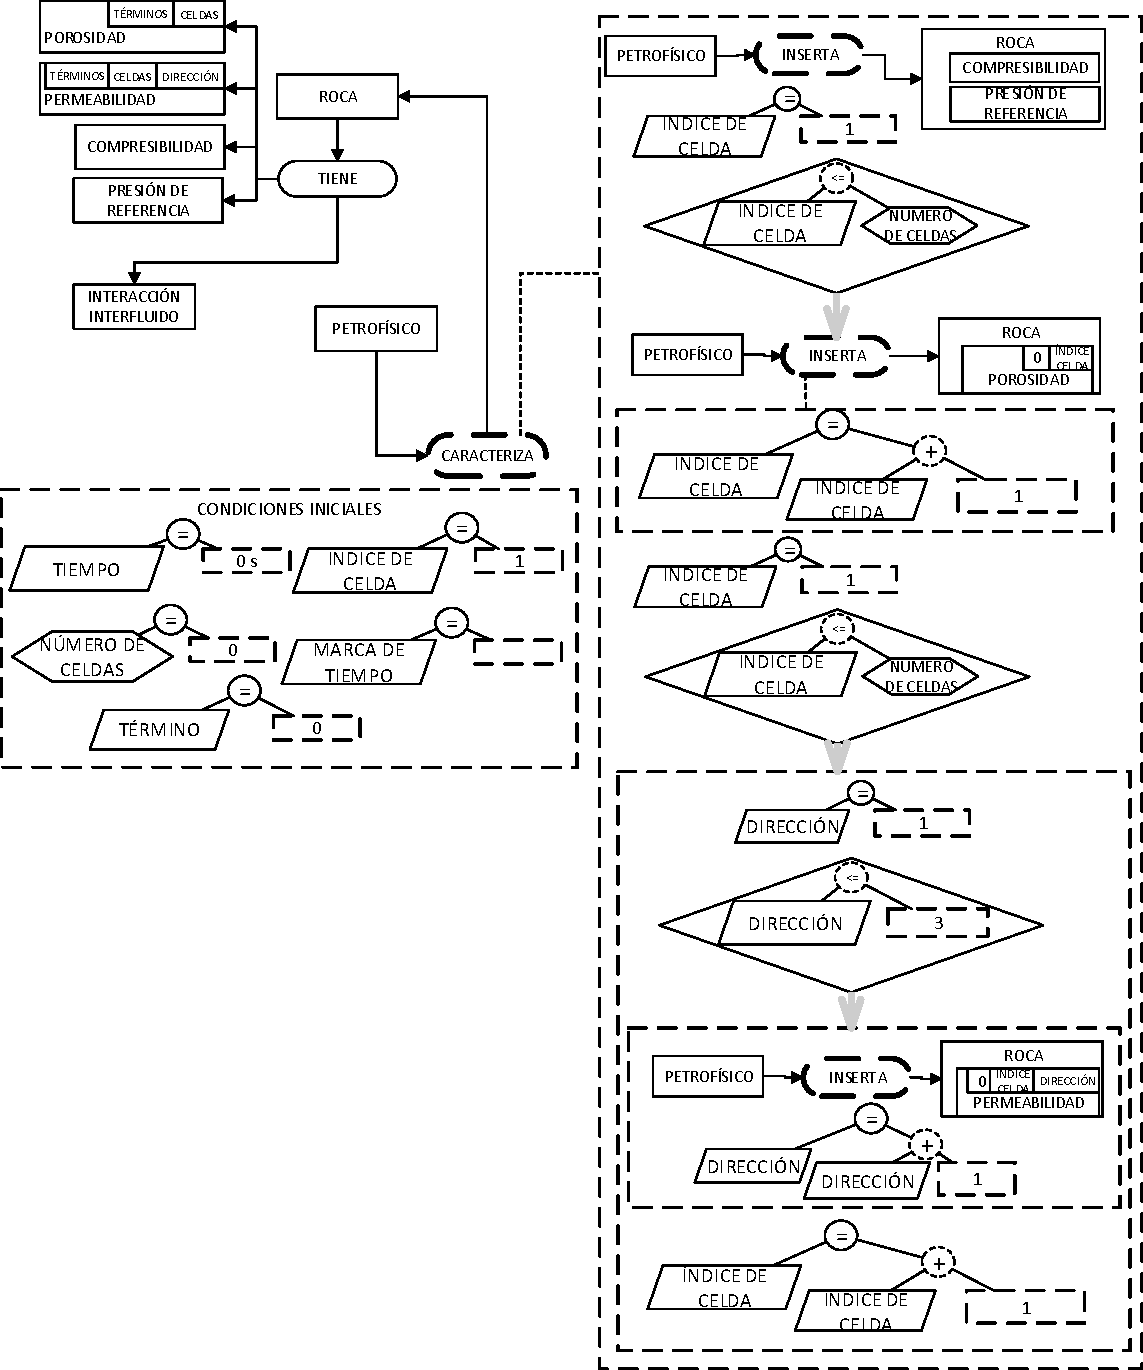
\includegraphics[width=1in]{Fig/Rock.pdf}\\ Ver figura \ref{fig:Rock}.\end{tabular}
			%
			%\caption[Elementos para la representación de Software Científico.]{Elementos para la representación de Software Científico. \citep{JCalle,norena2018det}.} \label{fig:RockTranslation}
		}
		&
		\begin{tiny}
			\begin{lstlisting}
			class Rock{
			private:
			
			double _reference_pressure;
			double _compressibility;
			std::vector<std::vector<std::vector<double>>> _absolute_permeability;   
			std::vector<std::vector<double>> _porosity;
			
			public:
			
			Rock(){};
			void characterize(const int& cells_number);
			void characterizeFromFile(std::ifstream& rock_reader,
			const int& cells_number);
			void porosity(const int term, const int cell_index,
			const double pressure);
			
			void updateProperties(const int& term);
			
			const double& porosity (const int term, const int cells_number) const {
			return _porosity[term][cells_number];
			};
			
			const std::vector<double>& absolutePermeability
			(const int term, const int cells_number) const {
			return _absolute_permeability[term][cells_number];
			};
			};
			
			\end{lstlisting}
		\end{tiny}
	\end{tabular}
	\label{tab:RockCode}
	\caption[Traducción a código del concepto Roca.]{Traducción a código del concepto Roca. Los autores.}
\end{table}

\begin{table}[h]
	\centering
	\begin{tabular}{cc}
		\parbox[c]{5em}{
			\begin{tabular}[c]{@{}c@{}}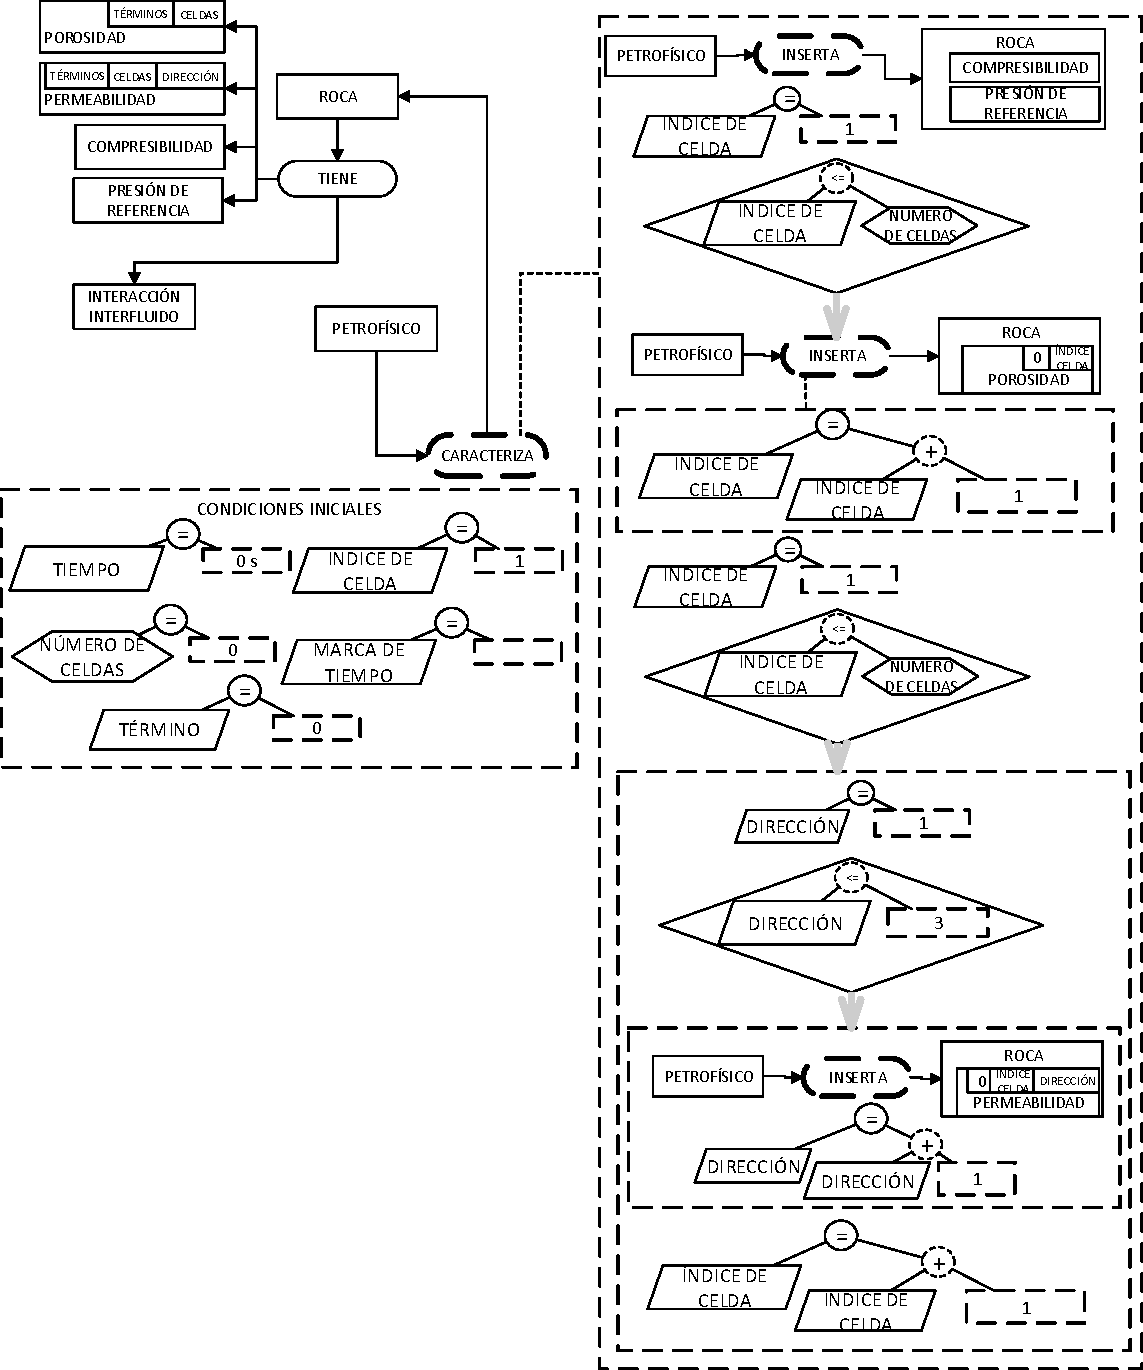
\includegraphics[width=1.5in]{Fig/Rock.pdf}\\ Ver figura \ref{fig:Rock}.\end{tabular}
				%
				%\caption[Elementos para la representación de Software Científico.]{Elementos para la representación de Software Científico. \citep{JCalle,norena2018det}.} \label{fig:RockTranslation}
		}
	 &
	\begin{tiny}
		\begin{lstlisting}
		void Rock::characterize(const int& cells_number){
		
		std::ostringstream ss = std::ostringstream();
		const std::string axisnames[3]={"x", "y", "z"};
		
		_absolute_permeability = std::vector<std::vector<std::vector<double>>>
		(1,std::vector<std::vector<double>>(cells_number,std::vector<double>(3)));
		_porosity              = std::vector<std::vector<double>>(1,std::vector<double>(cells_number));
		
		myRead(std::string("Please insert rock compressibility [1/Pa]"), _compressibility,
		 std::string("Please insert a valid input"));
		
		myRead(std::string("Please insert reference pressure [Pa]"), _reference_pressure,
		 std::string("Please insert a valid input"));
		
		for(int cellindex=0; cellindex<cells_number; ++cellindex){
		
		ss << "Please insert initial porosity for the "<< cellindex+1 << " cell [-]";
		myRead(ss.str(), _porosity[0][cellindex], std::string("Please insert a valid input"));
		ss.str("");
		ss.clear();
		
		
		};
		for(int cellindex=0; cellindex<cells_number; ++cellindex){
		for(int direction=0; direction<3;++direction){
		ss << "Please insert initial absolute permeability for the "<< cellindex+1
		<< " cell in direction " << axisnames[direction] << " [m2]";
		myRead(ss.str(), _absolute_permeability[0][cellindex][direction],
		 std::string("Please insert a valid input"));
		ss.str("");
		ss.clear();
		};
		};
		};
		
		\end{lstlisting}
	\end{tiny}
	\end{tabular}
\label{tab:RockCharacterizeCode}
\caption[Traducción a código de la relación dinámica ``Petrofísico caracteriza Roca''.]{Traducción a código de la relación dinámica ``Petrofísico caracteriza Roca''. Los autores.}
\end{table}

\begin{table}[h]
	\centering
	\begin{tabular}{cc}
		\parbox[c]{4em}{
			\begin{tabular}[c]{@{}c@{}}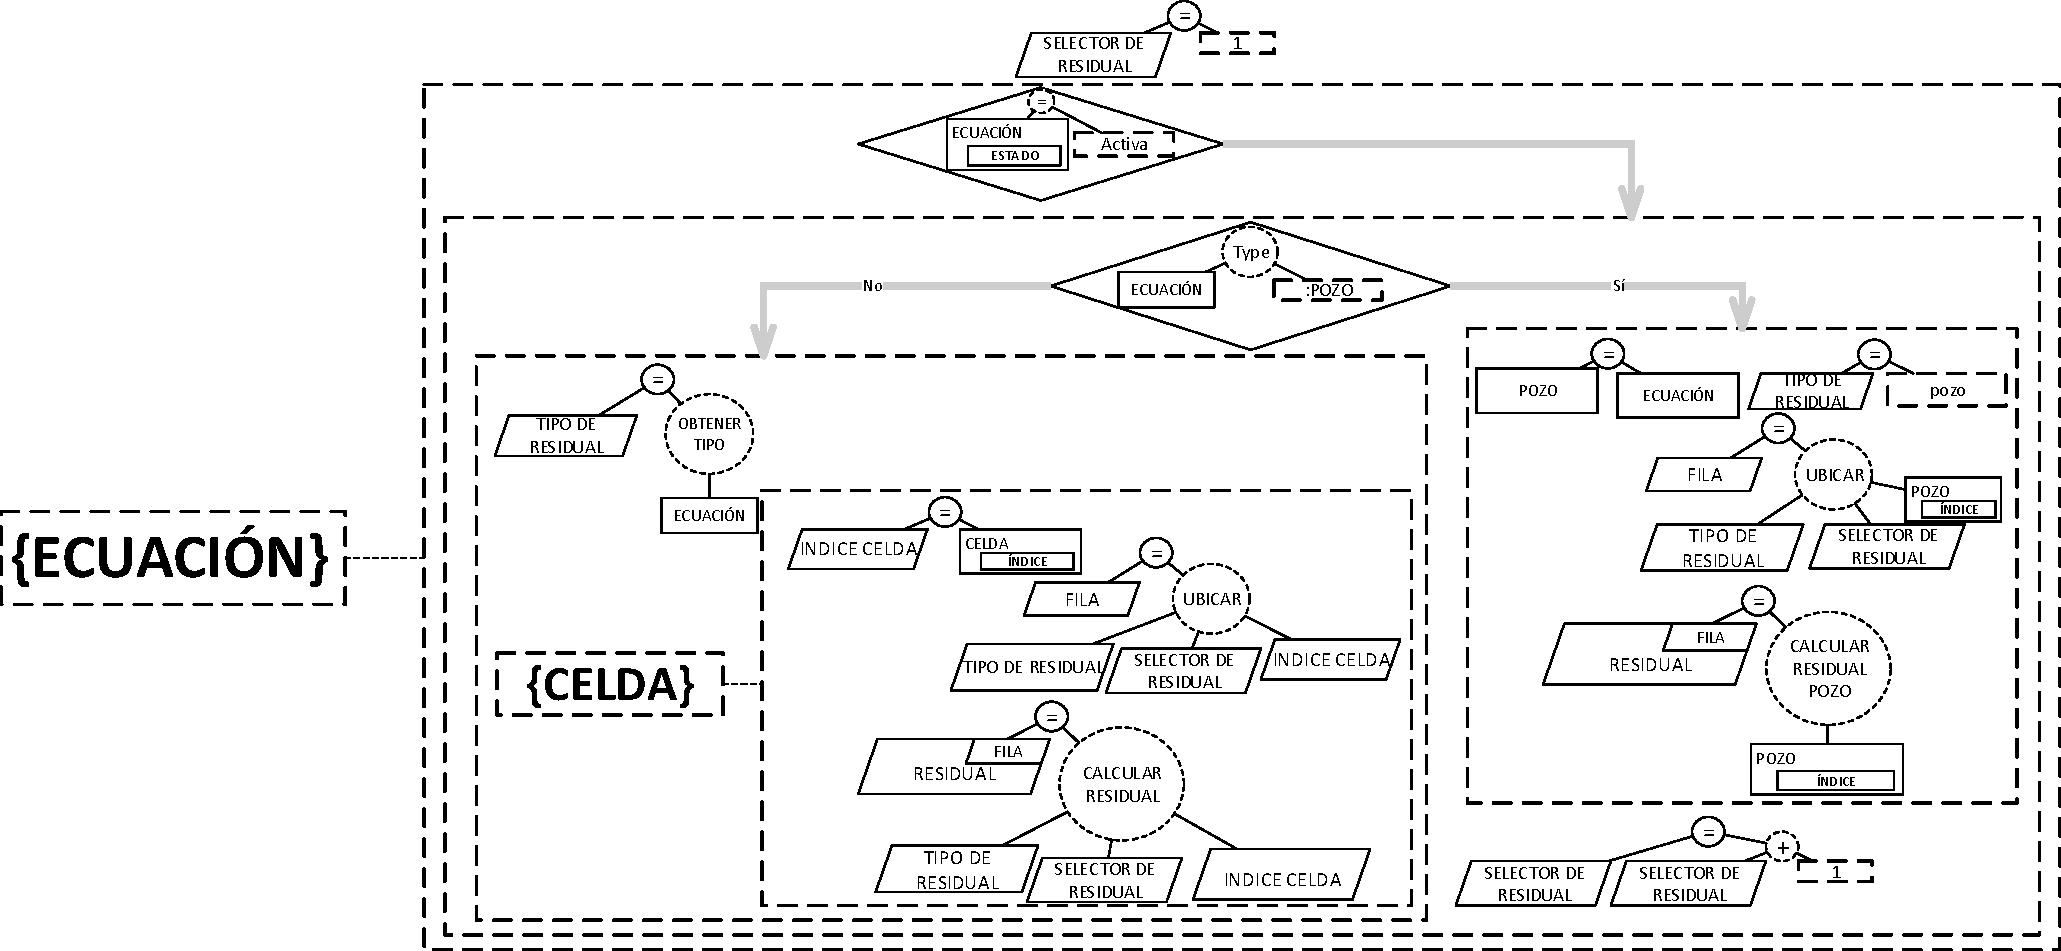
\includegraphics[width=2.5in]{Fig/Residual.pdf}\\ Ver figura \ref{fig:Residual}.\end{tabular}
			%
			%\caption[Elementos para la representación de Software Científico.]{Elementos para la representación de Software Científico. \citep{JCalle,norena2018det}.} \label{fig:RockTranslation}
		}
		&
		\begin{tiny}
			\begin{lstlisting}
			//Residual calculation
			residual_selector = 0;
			
			for(auto equation : equations){
			
			  if(equation->status()){
				
				if(equation->type() == typeid(Well).name()){
					
				  constexpr auto residual_type = "well";
				  auto residual_well = std::dynamic_pointer_cast<Well,Equation_Base>(equation);
					
				  row = locate(residual_type, residual_selector, residual_well->index());
				  _residual(row) = calculateWellResidual(term, residual_well);
						
				}else{
						
				  constexpr auto residual_type = "fluid";
				  auto residual_fluid = std::dynamic_pointer_cast<Fluid,Equation_Base>(equation);
						
				  for(auto cell = mesh.begin(); cell != mesh.end(); ++cell){
						
				    cell_index = (*cell)->index();
							
					row = locate(residual_type, residual_selector, cell_index);
							
					_residual(row) = 
					calculateResidual(term,*residual_fluid, mesh, *cell, rock, wells);
						
				  };
				};
					
				++residual_selector;
				
			  };
			};
			
			\end{lstlisting}
		\end{tiny}
	\end{tabular}
	\label{tab:ResidualCode}
	\caption[Traducción a código del cálculo de residual en el evento ``Presión del Fluido Varía''.]{Traducción a código del cálculo de residual en el evento ``Presión del Fluido Varía''. Los autores.}
\end{table}

\section{Simulación y resultados} \label{sec:results}

\subsection{Caso de literatura}

\subsection{Análisis de resultados}